\subsection{Was ist Deployment}

Wenn man vom Deployment spricht meint man die Bereitstellung von Software. Dies erfolgt meistens alles über halb- oder automatisierte Prozesse, mittels derer die Installation und Konfiguration der Softwarelösungen erfolgt. Im Deployment sind Aspekte wie die Installation, Konfiguration Aktualisierung und Wartung von Systemene enthalten.
Die meisten IT-Organisationen und Softwareentwickler führen regelmäßig Software-Updates und Patches mithilfe von teils vollautomatischen Prozessen durch. Es gibt verschiedene Arten von Deployment die jeweils verschiedene Risiken mit sich bringen. Dennoch wird überall dasselbe Ziel verfolgt: Die Verteilung von Software auf Computern für Endbenutzer.


\subsection{Verschiedene Arten von Deployment}

Grundsätzlich gibt es verschiedene Arten von Deployment. Diese werden prinzipell folgendermaßen kategorisiert:
    \begin{itemize}
    \item Traditionelles Deployment
    \item Virtuelles Depoyment
    \item Container Deployment
    \end{itemize}

\subsection{Traditionelles Deployment}

Früher wurde eine Anwendung auf einem physischen Server deployed. Damals sah das ganze folgendermaßen aus.

Es wurde ein physischer Server aufgesetzt auf welchem in Folge ein Betriebssystem installiert wurde auf welchen Die Software laufen soll. Im nächsten Schritt wurden auf dem Server benötigte Tools oder Packages wie zum Beispiel Node oder NPM installiert. Danach wurden alle Dateien der Software auf den Server kopiert. Im letzten Schritt wird dann die Anwendung auf diesem Server gestartet.


Solange nur eine einzige Anwendung auf diesem Server läuft, stellt dies kein Problem dar. Sogar im Gegenteil die Anwendung läuft dann sehr performant auf dem Server, da er jegliche Ressourcen die der Server frei hat benutzt. Sobald dann aber mehr als nur eine Anwendung auf einem Server laufen, führt dies zu Problemen, diese können sein:

\begin{itemize}
    \item Fehlende Ressourcen - auf einem physischen Server gibt es keine Möglichkeit, die Ressourcen für eine Applikation zu begrenzen. Eine Überlastung der Ressourcen kann somit den gesamten Server zum abstürzen bringen.
    \item Dateninkonsistenzen durch gemeinsam genutzten Speicher
    \item Es ist sehr teuer mehrere physische Server bereitzustellen.
\end{itemize}

\begin{figure}[h]
    \centering
    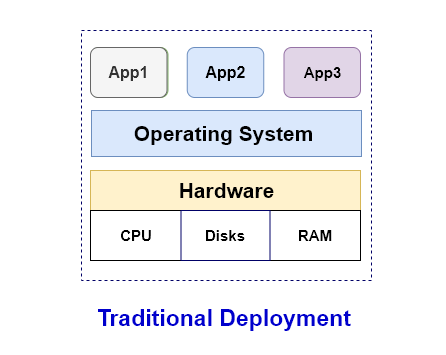
\includegraphics[width=0.8\linewidth]{pics/traditionelles-deployment.png}
    \caption{Traditionelles Deployment}
    \label{fig:enter-label}
\end{figure}


\cite{Traditional_vs_Container_vs_Virtuell_Deployment}


\subsection{Virtuelles Deployment}
Um diese Probleme zu lösen, begann man die Software virtuell zu deployen. In diesem Fall wurde eine virtuelle Maschine erstellt, die über ihre eigene Partition im Speicher und ein eigenes Betriebssystem verfügte. Somit gab es keine Probleme mehr mit einer Ressourcenüberlastung und die individuellen Aplikationen konnten auch isoliert werden. Dennoch traten auch einige Probleme bei dieser Lösung auf, darunter:

\begin{itemize}
\item Betriebssysteme weisen eine beträchtliche Datenmenge auf und benötigen mehrere Gigabyte Speicherplatz.
\item Es dauert sehr lange die virtuelle Maschine zu starten.
\item  Die Anwendung ist nicht portabel
\end{itemize}

\cite{Virtuelles_Deployment}

\subsection{Container Deployment}
Um auch die Probleme des virtuellen Deployments zu lösen, deployte man die Software nun in Containern.
Container sind in sich geschlossene, autarke Einheiten, die sämtlichen Anwendungscode und sämtliche erforderlichen Abhängigkeiten in sich tragen. Neben Docker, einem der prominentesten Werkzeuge zur Containerisierung von Anwendungen, stehen auch Alternativen zur Verfügung, darunter Lösungen wie Kubernetes und Podman. Container besitzen den Vorteil, dass sie sehr leichtgewichtig sind und daher in wenigen Sekunde oder Millisekunden gestartet werden können. Zudem sind Container im Gegenteil zu Virtuellen Maschinen äußerst portabel und skalierbar.



\subsubsection{Vorgang des Container Deployment}

Als erstes wird die gesamte Anwendung in ein Container Image verpackt. In diesem Image befindet sich der Anwendungscode, die Laufzeitumgebung und alle erforderlichen Abhängigkeiten wie zum Beipsiel Node oder NPM.

Als nächstes wird das erstellte Container Image in einem Container-Image-Repository wie Docker Hub registriert und gespeichert.

Danach müssen die Container Images bereitgestellt werden dies geschieht überlicherweise auf einem Container-Orchestrierungs-Framework wie Kubernetes oder Docker Swarm.

Als letzten Schritt muss der Container noch konfiguriert werden und mögliche Umgebungsvariablen gesetzt werden.

Wenn eine neue Version der Anwendung verfügbar ist, kann das Container-Deployment-Framework verwendet werden, um die Container schrittweise zu aktualisieren, ohne die Verfügbarkeit der Anwendung zu beeinträchtigen.


\begin{figure}[h!]
    \centering
    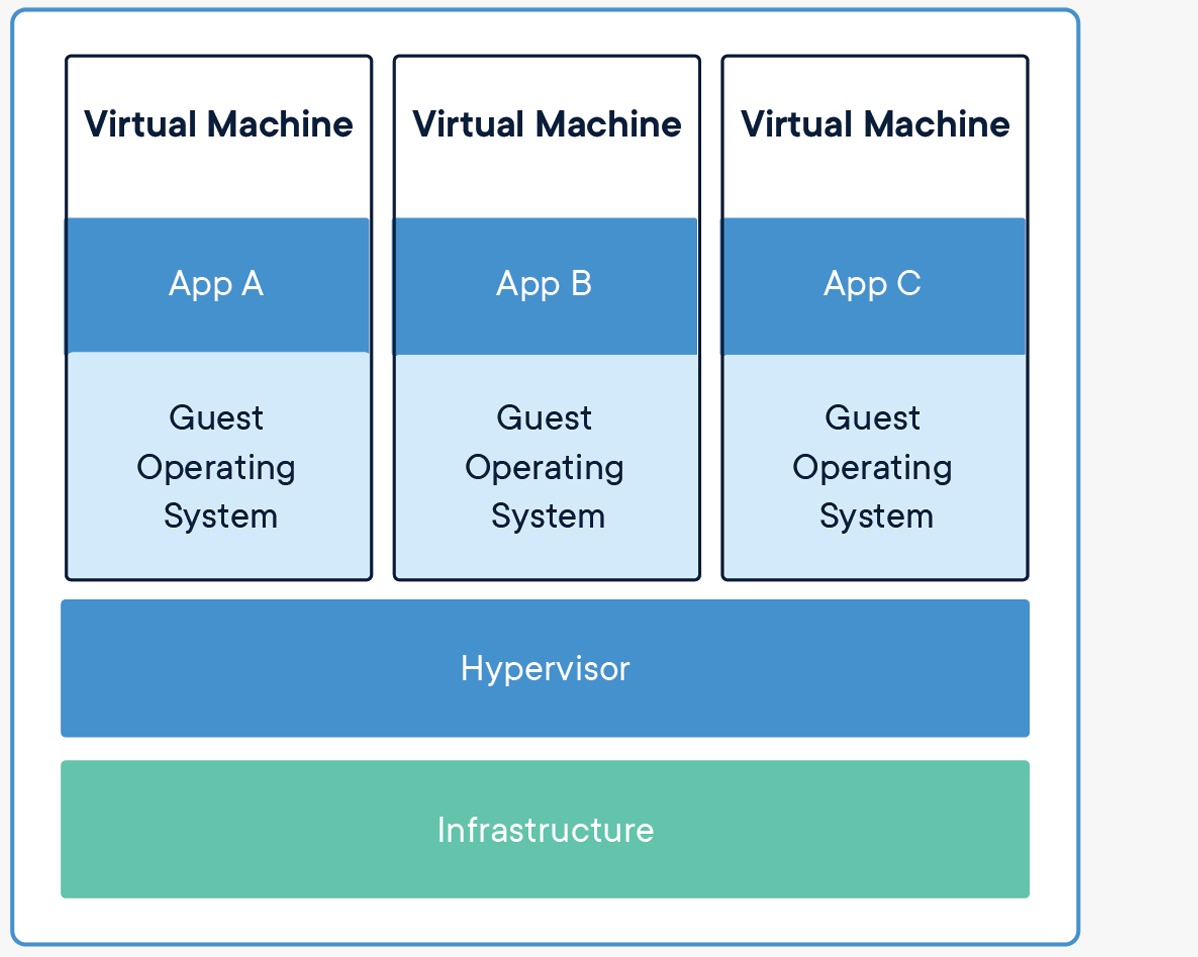
\includegraphics[width=0.8\linewidth]{pics/container_deployment.jpeg}
    \caption{Container Deployment}
    \label{fig:enter-label}
\end{figure}

\subsection{Umgebungsvariablen}

Umgebungsvariablen sind dazu da um die Anwendungsgeheimnisse und Konfigurationen zu speichern, die wenn nötig von der Anwendung abgerufen werden können. Umgebungsvariablen verleihen einer Anwendung mehr Dynamik. Somit kann von sehr schnell und einfach von internen auf externe Ressourcen umgeschaltet werden. Der Wert einer Umgebungsvariable kann aus verschiedenen Quellen stammen wie zum Beispiel Textdateien, Drittanbieter oder aufrufende Skripte. Das wichtigste an den Umgebungsvariablen ist aber, dass der Wert nicht statisch gecoded ist sondern wirklich dynamisch ist und je nach Umgebung verändert werden kann.

Es gibt verschiedene Arten von Umgebungsvariablen:

\begin{itemize}
    \item \textbf{Systemumgebungsvariablen}
        \newline
        Diese Art von Umgebungsvariablen befinden sich im obersten Verzeichnis und laufen unter dem Benutzerprofil. In den meisten Fällen werden sie vom Systemadministrator festgelegt. Das wohl häufigste Vorkommen einer Systemumgebungsvariable ist die "PATH" Variable. Diese legt fest in welchen Verzeichnissen gesucht wird, wenn ein Befehl in die Kommandozeile eingegeben wird.
        \cite{path_setzen}
        
    \item \textbf{Benutzer-Umgebungsvariablen}
        \newline
        In diesen Variablen wird zum Beispiel der Pfad zu einer lokal installierten Bibliothek gespeichert, welche nur von manchen Benutzern verwendet wird. Für Änderungen an dieser Variable wird der Systemadministrator nicht benötigt. Diese Variablen sind sehr hilfreich um lokale Änderungen nur für einen Benutzer gültig zu machen.
    \item \textbf{Laufzeit-/Prozessumgebungsvariablen}
        \newline
        Auf diese Art von Umgebungsvariablen hat der Benutzer mehr oder weniger keinen Einfluss. Die Lebensdauer dieser Umgebungsvariablen ist durch den übergeordneten Prozess begrenzt, der sie erstellt hat.
        Sollte es aber den speziellen Fall geben, das der Benutzer Einfluss auf die Laufzeitumgebungsvariablen braucht, dann kann er diese im Terminal-Skript erstellen.
\end{itemize}

Im Falle diese Diplomarbeit wurden Umgebungsvariablen hauptsächlich verwendet um die Sicherheit aufrecht zu erhalten und Datenbankbezogene Informationen oder API - Keys darin zu speichern.

\subsubsection{.env-Dateien}
In dieser Diplomarbeit wurden .env Files verwendet um die Umgebungsvariablen zu speichern. Die Anwendung ist sehr simpel. Es muss im Stammverzeichnis des Projektes eine .env Datei angelegt werden in dieser können nach folgendem Schema die Umgebungsvariablen definiert werden:
\begin{verbatim}
    VAR_UNO=SOME_KEY_HERE
    VAR_DOS=SOME_OTHER_KEY_HERE
\end{verbatim}

Wenn diese Variablen von der Anwendung benötigt werden, sucht diese danach und lädt sie während der Laufzeit ins Programm. 
Es können allerdings auch mehrere Dateien erstellen werden für mehrere Umgebungen z.B
\begin{verbatim}
    .env.dev -> Fuer die Developement Umgebung
    .env.prod -> Fuer die Production Umgebung
\end{verbatim}

Wichtig ist außerdem noch die .env Dateien nicht in eine Versionskontrolle wie Github aufzunehmen. Wenn ein spezielles Schema definiert wurde welches auch für andere Entwickler wichtig ist erstellt man in den meisten Fällen eine .env.template Datei und definiert hier das Schema folgendermaßen:

\begin{verbatim}
    VAR_UNO= # Your value here
    VAR_DOS= # Your value here
\end{verbatim}

Somit ist das Schema bekannt aber vertrauliche Werte werden nicht in die Versionskontrolle mit aufgenommen.


\cite{Umgebungsvariablen}




\subsection{Docker}

Docker wurde erstmals im März 2013 von dotCloud veröffentlicht und nutzt den Linux-Kernel und seine Ressourcenkontrollmechanismen wie Cgroups und Namespaces, um Prozesse zu isolieren, wodurch sie in voneinander unabhängigen Umgebungen ausgeführt werden können. Dieser fundamentale Aspekt der Container-Technologie ermöglicht die parallele Ausführung mehrerer Prozesse und Anwendungen in isolierten Containern. Dies steigert die Effizienz Ihrer Infrastruktur, ohne dabei die Sicherheitsvorteile zu vernachlässigen, die sich aus der Nutzung separater Umgebungen ergeben.

Container-Tools wie zum Beispiel Docker arbeiten auf mit einem imagebasierten Deployment-Modell. Dies erleichtert der Anwendung die Nutzung von gemeinsamen Ressourcen und Services mit sämtlichen Abhängigkeiten.

Mit Docker ist es möglich einen Teil einer Anwendung zu aktualisieren oder reparieren ohne die gesamte Anwendung deaktivieren zu müssen. Außerdem besitzt Docker eine Rollbacking, also das zurücksetzen auf die vorherige Version.

\cite{Vorteile_Nachteile_Docker}
\cite{Was_ist_Docker}




